\chapter{\IfLanguageName{dutch}{Stand van zaken}{State of the art}}%
\label{ch:stand-van-zaken}

% Tip: Begin elk hoofdstuk met een paragraaf inleiding die beschrijft hoe
% dit hoofdstuk past binnen het geheel van de bachelorproef. Geef in het
% bijzonder aan wat de link is met het vorige en volgende hoofdstuk.

% Pas na deze inleidende paragraaf komt de eerste sectiehoofding.

%\lipsum[7-20]

\section{Wie is Lockit Rentals}%
\label{sec:lockitRentals}


Lockit Rentals is een naam onder het bedrijf VD Group BV. Deze is opgericht op 6 november 2019 door Sébastien Vandenhouten en Wannes Van Dorpe met als doel lockers te verhuren op evenementen. Enkele maanden na de oprichting begon de covid-19 crisis die de volledige sector tot stilstand deed komen. Na de crisis werd er direct geïnvesteerd in nieuwe lockers. Niet de gewone traditionele lockers, maar speciale technologische lockers die nog niet beschikbaar waren in België. De lockers werden in een mum van tijd omgebouwd tot QR-smart locker units met daarin lockers. Zo zijn er in het voorjaar van 2022, 13 units geproduceerd door Lockit Rentals. Op de dag van vandaag wordt er ijverig gezocht naar nieuwe investeerders om hun vloot van units uit te breiden.

Er zijn verschillende manieren om smart lockers systemen te gaan produceren. Hieronder volgt een opsomming van de verschillende smart lockers systemen elk met hun eigenschappen. Deze methodes zijn opgesteld door Lockit Rentals om hun marktonderzoek te starten.
\\
\textbf{Pincode:}
\begin{itemize}
    \item Kan vergeten worden
    \item Manuele verkoop mogelijk
    \item 100\% online verkoop mogelijk
    \item Trage verwerking bij openen van locker (pincode moet manueel worden ingetypt)
    \item Spieken is mogelijk waardoor er risico’s tot diefstal    
\end{itemize}
    
\newpage
\textbf{Rfid Badge:}
\begin{itemize}
    \item Kan verloren gaan
    \item Manuele verkoop mogelijk
    \item Geen online verkoop mogelijk
    \item Snelle verwerking bij openen locker (scan en go)
    \item Spieken is niet mogelijk
    \item Fysiek object nodig + aankoop kost van badges    
\end{itemize}

\textbf{QR  code:}
\begin{itemize}
    \item Kan niet vergeten worden (kan ook niet onthouden worden)
    \item Manuele verkoop mogelijk
    \item 100\% online verkoop mogelijk
    \item Snelle verwerking bij openen lockers (scan QR-code en go)
    \item Spieken is niet mogelijk
    \item Technisch een veelvoud aan vereenvoudigingen mogelijk    
\end{itemize}

Uit deze korte opsomming van eigenschappen heeft Lockit Rentals besloten om zich te richten op het maken van lockers die openen op basis van een correcte QR code. Het gebruik van een QR code is vandaag de dag ook geen onbekend terrein. Door het mainstream maken van QR codes in betalingen, doorlinken van websites, covidsafe app, etc. zijn veel mensen al eens in aanraking gekomen met een QR-code \autocite{Belle2023}. Het gebruik van een QR code voor het openen van lockers is de logische stap voorwaarts \autocite{Lo2014}.
Uiteraard zijn ze niet de enige die smart locker systemen op de markt hebben. Enkele bedrijven die hier ook bij aanschuiven zijn, mobile lockers, LockerKing en Rental Group.

\section{Hoe zijn de QR-units opgebouwd?}%
\label{sec:QR-units}
De smart locker systemen zijn toegankelijk met een geldige toegangscode die voorgesteld wordt als een QR-code. Het systeem bestaat uit verschillende soorten technologieën en elektronische componenten. De combinatie van hardware en software die nauw met elkaar samenwerken, vormen gezamenlijk één QR-unit \autocite{Jadhav2016} . De units hebben enkel 230 volt nodig om volledig operationeel te zijn. 

De hardware bestaat uit mechanische onderdelen zoals een deurslot \ref{fig:lockerSlot}, het volledige frame van de unit maar ook uit elektronische onderdelen zoals een camera, Raspberry Pi, scherm, etc. De mobiele applicatie waar de QR-codes kan verkocht worden en zo ook genereren, heeft geen verband met de interne werking van een QR-unit. Het enige dat de QR-unit nodig heeft, is een correct opgebouwde QR-code. Hiermee krijgt de festivalganger toegang tot zijn/haar gehuurde locker.

Elke unit bevat 128 lockers verspreid over 4 kasten zoals te zien op figuur \ref{fig:lockerUnit}. De Locker units zijn waterdicht en dus optimaal voor plaatsing in niet overdekte locaties. Eén locker kast bevat 24 lockers, 4 grote die zich op de bovenste rij bevinden. De 20 overige zijn een iets kleiner formaat en situeren zich onderaan. De lange zijden van een QR-unit zijn uitklapbare luiken met aan elke kant twee kasten. Er zijn 4 kasten per unit aanwezig wat een totaal geeft van 128 lockers voorgesteld op figuur \ref{fig:lockerUnit} en  \ref{fig:lockerUnit2}.

\begin{figure}[h]
    \centering
    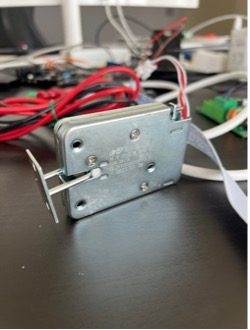
\includegraphics[height=7cm]{F1_lockerSlot.jpg}
    \captionsetup{justification=centering, singlelinecheck=false}    
    \caption{Een locker slot.}
    \label{fig:lockerSlot}
\end{figure}}

\begin{figure}[h]
    \centering
    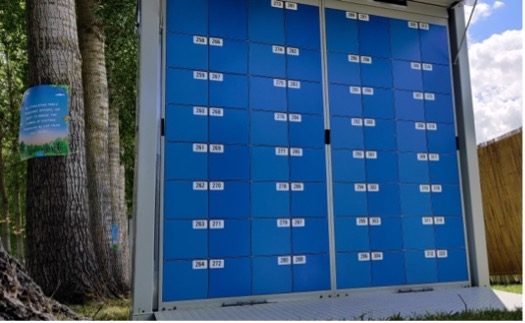
\includegraphics[height=6cm]{F2_lockerUnit.jpg}
    \captionsetup{justification=centering, singlelinecheck=false}    
    \caption{Reële weergave van een locker unit.}
    \label{fig:lockerUnit}
\end{figure}

\begin{figure}[h]
    \centering
    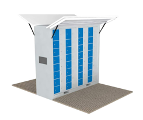
\includegraphics[height=7cm]{F3_lockerUnit2.png}
    \captionsetup{justification=centering, singlelinecheck=false}    
    \caption{Een uitgetekende weergave van een locker unit.}
    \label{fig:lockerUnit2}
\end{figure}}

\section{Hoe is een QR-code opgebouwd?}%
\label{sec:opbouwQR-code}

Een QR-code is een machinaal leesbaar optisch label met informatie over het bijhorende product \autocite{Chang2014}. In deze context wordt het product als toegangscode gebruikt. QR-code staat voor Quick Response code en is een matrix van de welbekende streepjes code \autocite{Tiwari2016}. Het is een tweedimensionale code die informatie zoals tekst, URL of andere data bevat  \autocite{Shin2012} \autocite{Baharav2013}. In ons geval is het dus informatie die toebehoort bij een overeenkomstige locker. De QR-code is zodanig ontworpen dat ze door een smartphone uitgelezen kan worden aan hoge snelheden \autocite{Tiwari2016}. Dit maakt het optimaal als de QR-code gebruikt wordt als toegangscode \autocite{Narang2012}. De grootte van de QR-code kan aangepast worden naarmate de hoeveelheid data die hierin gestockeerd moet worden \autocite{Tiwari2016}. 
\\
Een QR-code wordt opgebouwd en voorgesteld als een vierkant \autocite{Fujita2011}. Hierrond bevindt zich een witte omranding. Dit vormt een contrast zodat de QR-scanner minder moeite heeft om de oppervlakte uit te lezen \autocite{Wang2015}. Dit is 1 van de 7 cruciale eigenschappen. Plaats markeringen zijn aanwezig om de scanner een duiding te geven hoe de code is gepositioneerd. Uitlijnmarkeringen hebben eveneens dezelfde functie maar deze zijn meer van toepassing bij grote QR-codes. De QR-code bevat timing patronen, dit zijn lijnen die de scanner vertellen hoe groot de data matrix is. De twee belangrijkste elementen van een QR-code zijn gegevens en foutcorrectiesleutels. Hierin zit de data gecapteerd inclusief de informatie hoe het algoritme moet omgaan met fouttolerantie \autocite{Tiwari2016}  \autocite{Petrova2016}  \autocite{Li2018}). Een visuele weergave is tezien op \ref{fig:voorstellingQR}. 
De fouttolerantie is doorslaggevend indien de QR-code gebruikt wordt als toegangscode \autocite{Tiwari2016}.  De fouttolerantie kan ingesteld worden door configuratie toe te passen. Het kan ingesteld worden op vier levels beginnend bij fouttolerantie van 7\% tot 30\% \autocite{Tiwari2016}.

\begin{figure}[h]
    \centering
    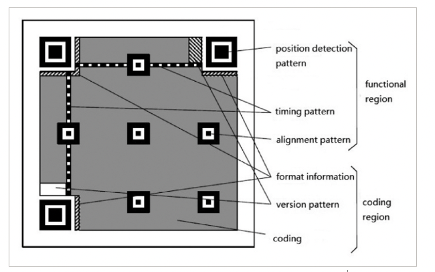
\includegraphics{F4_voorstellingQrCode.png}
    \captionsetup{justification=centering, singlelinecheck=false}    
    \caption{Een technische voorstelling van een QR-code.}
    \label{fig:voorstellingQR}
\end{figure}}

De voordelen van de QR-codes vormen een duidelijk beeld waarom Lockit Rentals voor deze technologie gekozen heeft. Niet enkel naar functionaliteit en flexibiliteit toe maar eveneens is het een makkelijk traceerbare tool. Bij verkoop van QR-codes kan men een overzicht opmaken hoeveel QR-codes er effectief gegenereerd zijn. Op basis van deze gegevens kunnen verkoopcijfers makkelijk berekend worden. 

De kans op diefstal wordt ook alsmaar kleiner als de toegangscode bestaat uit elementen die niet waarneembaar zijn \autocite{Baharav2013}. Hoe minder de persoon in kwestie weet over de code hoe moeilijker deze is om door te geven aan anderen ook al is het niet hun intentie.
\newpage
\subsection{Opbouwen van QR-codes voor verkoop}%
\label{sec:opbouwQR-codeVerkoop}

De applicatie kan meerdere versies van QR-codes genereren elk met hun eigen doel en eigenschappen. Zo bestaan er QR-codes die de software automatisch updaten of een universele QR-code die automatisch alle lockers kan openen. Deze functionaliteit wordt gebruikt voor de lockers te controleren na elk evenement. 

Hoewel een QR-code een standaard grafische voorstelling is, kan de grootte van een code verschillen. Wanneer een code groter is, ontstaat er meer witruimte tussen de pixels \autocite{Li2018}. Hierdoor kan de camera de code makkelijker en sneller scannen \autocite{Karrach2020}. Ook de foutcorrectie zorgt ervoor dat de resolutie vergroot zal worden. Hoe groter de resolutie van de QR-code hoe meer data gestockeerd kan worden \autocite{Chow2016}. 

De reservatie en tot stand brengen van een QR-code zijn twee aparte concepten. Het systeem is geschreven op basis van flexibiliteit en uitbreidbaarheid.

\subsubsection{Aanmaken reservatie en betalingsverzoek voor verkoop}%
\label{sec:opbouwQR-codeVerkoop1}

\textit {De toelichting die hieronder weergeven wordt, is een vereenvoudigde voorstelling van de effectieve implementatie. Dit onderdeel van de toepassing is niet het hoofdonderwerp van deze bachelorproef, op deze analogie wordt niet verder ingegaan.}

De gegevens van de klant worden opgevraagd als hij/zij een QR-code wenst te kopen. Aan de hand van deze gegevens wordt er een gebruikersaccount automatisch aangemaakt en worden de gegevens bijgehouden. Deze aanpak maakt het mogelijk om nadien een koppeling te leggen tussen lockernummer en gebruiker. 

\begin{listing}[!ht]
    \begin{minted}{c}
        #include <stdio.h>
        int main() {
            printf("Hello, World!"); /*printf() outputs the quoted string*/
            return 0;
        }
    \end{minted}
    \caption{Hello World in C}
    \label{listing:2}
\end{listing}

